\documentclass[Softwaredesign/Softwaredesign_main.tex]{subfiles}
\begin{document}
\subsection{Design af RPiApp - USER SPACE}
Beer Pong er et event baseret spil. Det omhandler masser af asynkrone handlinger; når der rammes ned i en kop, indsættelse af mønt mm. Det er således utroligt vigtig at vores system kan opfange alle disse asynkrone events. Selvom alle handlingerne fra brugeren er asynkrone, ønsker vi stadigt at interagere med handlingerne sekventielt. Dette er en vigtig faktor, da hvis bruger laver to event handlinger inden for en kort tidsrammer, skal vi sikre at systemet når at reagere på begge handlinger. En af måderne for at opnå dette er reaktiv programmering: vi ønsker at opdatere vores system med det samme brugeren interagere med det. 
\\Reaktv programmering er dog blot en af de ting, som er nødvendigt for vores system. En anden er håndtering af de asynkrone events. Vi skal sikre os, at når en enhed en tilstand af foranding (fx en bruger har fjernet en kop), at vi håndtere dette korrekt. Der kan også opstå et tilfælde, hvor to enheder (fx Playersides) sender en asynkron besked til RPi samtidigt. Her skal det være muligt at afhandle begge beskeder. Dette problem kan løses ved 'event driven' arkitektur. 

\textbf{Event driven arkitektur}
\\Et event drevet system reagere ud fra signaler og tilstande fra aktører/delsystemerne\footnot{Delsystemer er repræsenteret i form af boundary klasserne i RPiApp} i systemet. Her bruges en bus til at håndtere events i en sekventiel orden, således intet går tabt og det ikke kan forstyrres fra andre delsystemer. 
\\En måde at håndtere signalerne imellem delsystemerne er brugen af MsgQueue. MsgQueue er en klasse, som gør det muligt at sende og modtage brugerdiffineret beskeder uden de kan påvirkes, opfanges eller forstyrres af andre tråde eller lignende. De brugerdefineret beskeder laves i form af nedarvninger af klassen Message. Da beskederne er brugerdefineret kan vi designe dem således de kan indeholde den information vi ønsker, om det skal være en int, objekt af klasse eller lignende.\footnote{MsgQueue og Message klasserne er udarbejdet i ISU-faget}. 
\\MsgQueue indeholder også et objekt af en STL Queue. Dette betyder at når en besked modtages eller sendes er strukturen FIFO (First in, first out). Dette betyder at selvom beskederne er asynkrone, så vil de behandles sekventielt i 'køen'. Hvert delsystem får et MsgQueue objekt, således de kan kommunikere med hinanden. 

\begin{figure}[H]
    \centering
    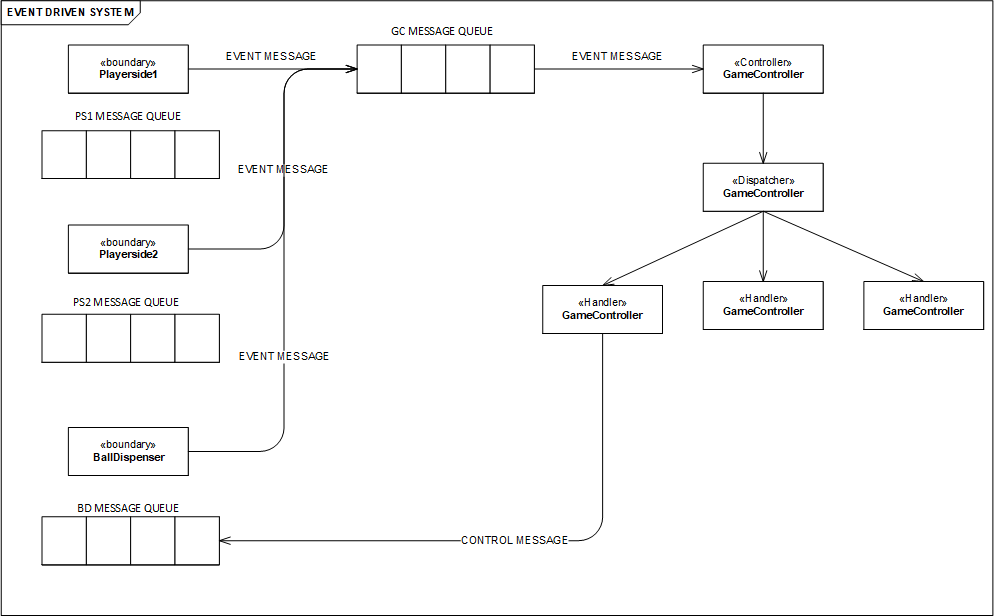
\includegraphics[width=0.8\textwidth]{Softwaredesign/RPiApp/graphic_RPi/EDS.png}
    \caption{Skitse af event drevet system (Version 1, ikke færdig)}
    \label{fig:EDS}
\end{figure}

\textbf{Delsystemer og tilhørende tråde}
\\For hver boundaryklasse tildeles en tråd - for boundaryklassen BallDispenser og Playerside tildeles en tråd til at læse og skrive, da når funktionen readPlayerside() kaldes sover funktionen og dermed også tråden. Vi ønsker stadig at kunne sende til Playerside og må derfor have en sideløbende tråd til at skrive til den. Alle tråde skal konstant checke deres MsgQueue objekt (Deres besked kø) for information. Når en besked modtages, afhandles den via en 'dispatcher'. Nedenfor ses et eksempel på en tråd.
\\Design example for thread function. \footnot{Idéen af dette design er taget fra ISU undervisning: Thread_Communication}
\begin{lstlisting}
void * threadFunction(void *)
{
    while(systemisactive)
    {
        unsigned long id;
        Message * msg = MessageQueueObj_.recieve(id);
        Dispatcher(msg, id);
        delete msg; 
    }
}
\end{lstlisting}


\texbf{Dispatchers og handlers}
\\En dispatcher er en overall event handler. Den bruges til at håndtere den besked som tråden modtagere gennem dens besked kø. Der 'modtages' to parametre fra recieve()-funktionen: et id repræsentere den service handleren skal tilbyde og beskeden, som er en nedarvet brugerdefineret objekt af klassen Message (Den kan indeholde forskellige parametre i sig selv, hovedsageligt information som skal veksle mellem trådene). Ud fra parameteren 'id' vurderes hvilke service, som skal udføres. Dispatcheren 'aktiverer' derefter de korrekte event handlers og videregiver message, hvis dette er relevant. 
\begin{figure}[H]
    \centering
    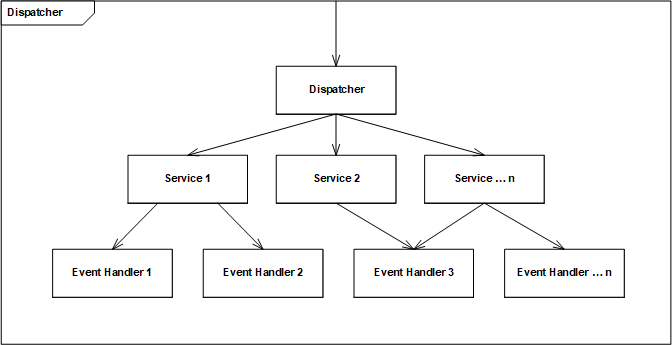
\includegraphics[width=0.8\textwidth]{Softwaredesign/RPiApp/graphic_RPi/dispatch.png}
    \caption{Skitse af dispatcher, services og eventhandlers (Version 1, ikke færdig, måske heller ikke så relevant)}
    \label{fig:dispatch}
\end{figure}
Nedenfor findes et kode eksempel på en dispatcher og hvordan en id og beskeder afvikles: 
\begin{lstlisting}
void dispatcher(unsigned long msgID, Message * msg)
{
    switch(id) 
    {
        case SERVICE 1 :
        {
            EventHandler1(static_cast<InheritedMessageType *>(msg)); 
        }
        break;
        
        case SERVICE 2 : 
        {
            EventHandler2(); 
            EventHandler3(static_cast<InheritedMessageType *>(msg));
        }
        break;
        default : //Error handling
    }
}
\end{lstlisting}


%Kode:
\begin{lstlisting}
obj_->getMsgQueue()->send(GameController::ID_GAME_START, msg); 
\end{lstlisting}

\end{document}